\subsection{Program}
To tie everything together we have made the program class which handles the state of the game. This class is a classic state machine.

\begin{lstlisting}[caption={A tick of the game},label={lst:tick},frame=tlrb, language=C++]{Name}
void tick() {
	switch(state) {
		case(program_state::Idle) : idle_tick(); break;
		case(program_state::Playing) : playing_tick(); break;
		case(program_state::Win) : win_tick(); break;
		case(program_state::GameOver) : game_over_tick(); break;
		default: break;
	}
}
\end{lstlisting}

As seen in Listing~\ref{lst:tick}, we have different behavior depending upon which state we are in. The tick decides what to do depending on the state, the game is in. 

\begin{figure}
\centering
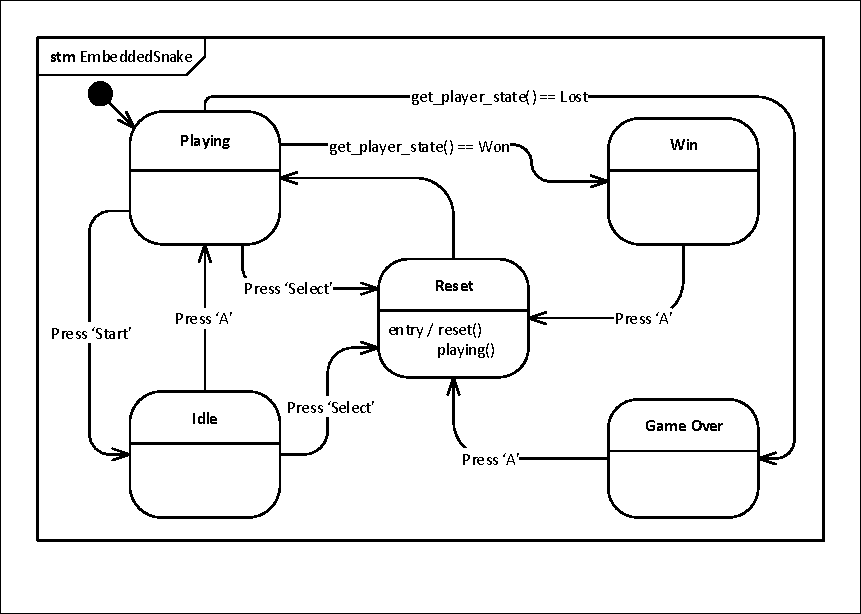
\includegraphics[width=0.7\textwidth, trim={5mm 10mm 5mm 5mm}, clip]{implementation/stm}
\caption{Flowchart of basic Snake game}
\label{fig:flow}
\end{figure}

As seen in Figure~\ref{fig:flow}, we have four states and a reset state, that only ensures, we get reset properly. The reason for the START button pausing the game and the A button resuming is that we do not check whether the button was pressed in the previous tick.  If multiple button presses are transmitted, the game will forward in one direction.

